\chapter{Introduction: Cities and networks}
%Why study cities? 

\epigraph{Cities have the capability of providing something for everybody, only because, and only when, they are created by everybody.}{Jane Jacobs, \textit{The Death and Life of Great American Cities} (1961, p. 238)}

As an architect my first approach to study cities was from the buildings' perspective, understanding how, by building, we delimit and shape spaces that model experiences in the city~\cite{gehl1971life}. These buildings are fundamental to define public spaces, mobility infrastructures, and even services that enable us to inhabit the \textit{ville}~\cite{sennett2018building}. The way we shape the city has an influence on how we inhabit it. Thus, understanding its infrastructures is fundamental to understanding and planning better cities for an increasingly complex future. Especially, when tackling urban mobility challenges, the way we plan, build and use mobility infrastructures is fundamentally entangled with the livability of our cities.

When thinking about urban infrastructures, my first approach was to use drawings and blueprints. These tools are useful to understand, and plan urban mobility. They provide a way to move from the physical structure of cities to a more concrete way to represent them. These maps and blueprints are a useful tool to abstract the reality and make it more manageable. Of course, one must be cautious when building such maps: at the end they are a representation of the territory, not the territory itself~\cite{borges1961hacedor}. Maps and blueprints provided me with an overview of cities and tools to move between scales.

As I studied cities, I became interested in getting to understand the relation between different transportation modes, and how cities and their mobility infrastructures could be studied using large scale data systematically. This curiosity led me to the complex systems field, and the use of network science to study cities. 

In this thesis I present the work of four years of research in the intersection of cities and complex networks. From this point onward I speak in plural, as even though I am the one presenting it, my research has been done in collaboration with co-authors. 

%Lit review
\section{Cities and network science}


As a complex system, a city offers a fertile study ground from multiple perspectives. Urban studies have engaged in analyzing different aspects of urban life, from sociological perspectives to more technical ones such as engineering. Due to this diversity and overlapping approaches, the ``science of cities'' is inherently interdisciplinary.

In cities, interdisciplinarity goes beyond the application of tools and methods borrowed from one discipline to study a different object. Indeed, when we think and engage in the analysis of urban phenomena, we encounter a multitude of approaches without a single dominant one. When studying cities one can start taking apart its pieces and analyze them separately. For instance, buildings, roads, and functions can all be studied without taking into consideration the rest of the pieces. However, following this approach misses the interactions between the pieces. 

Cities are more than the sum of their parts. It is in the interactions between its different pieces and components where one can find the richness of cities and the spark of urban life~\cite{Jacobs1961Death}. In a mostly urbanized world, capturing these relations is fundamental to not only understand the cities, but to plan better and more human ones. As cities evolve through time they grow and change, as defined by Manuel Castells, contemporary cities are a ``space of flows''~\cite{castells1989informational}. 

To capture these changes and flows, the complex system framework can be used. Indeed, this approach has enabled new urban research opportunities, such as the characterization of urban areas as fractals~\cite{batty1996preliminary} to investigate the cities' spatial organization, and their growing processes and evolution~\cite{makse1995growth}. However, to be able to capture the relations and interactions between places one can study cities as a system. To do so, we can use networks.

\begin{figure*}[th!]
	\centering
	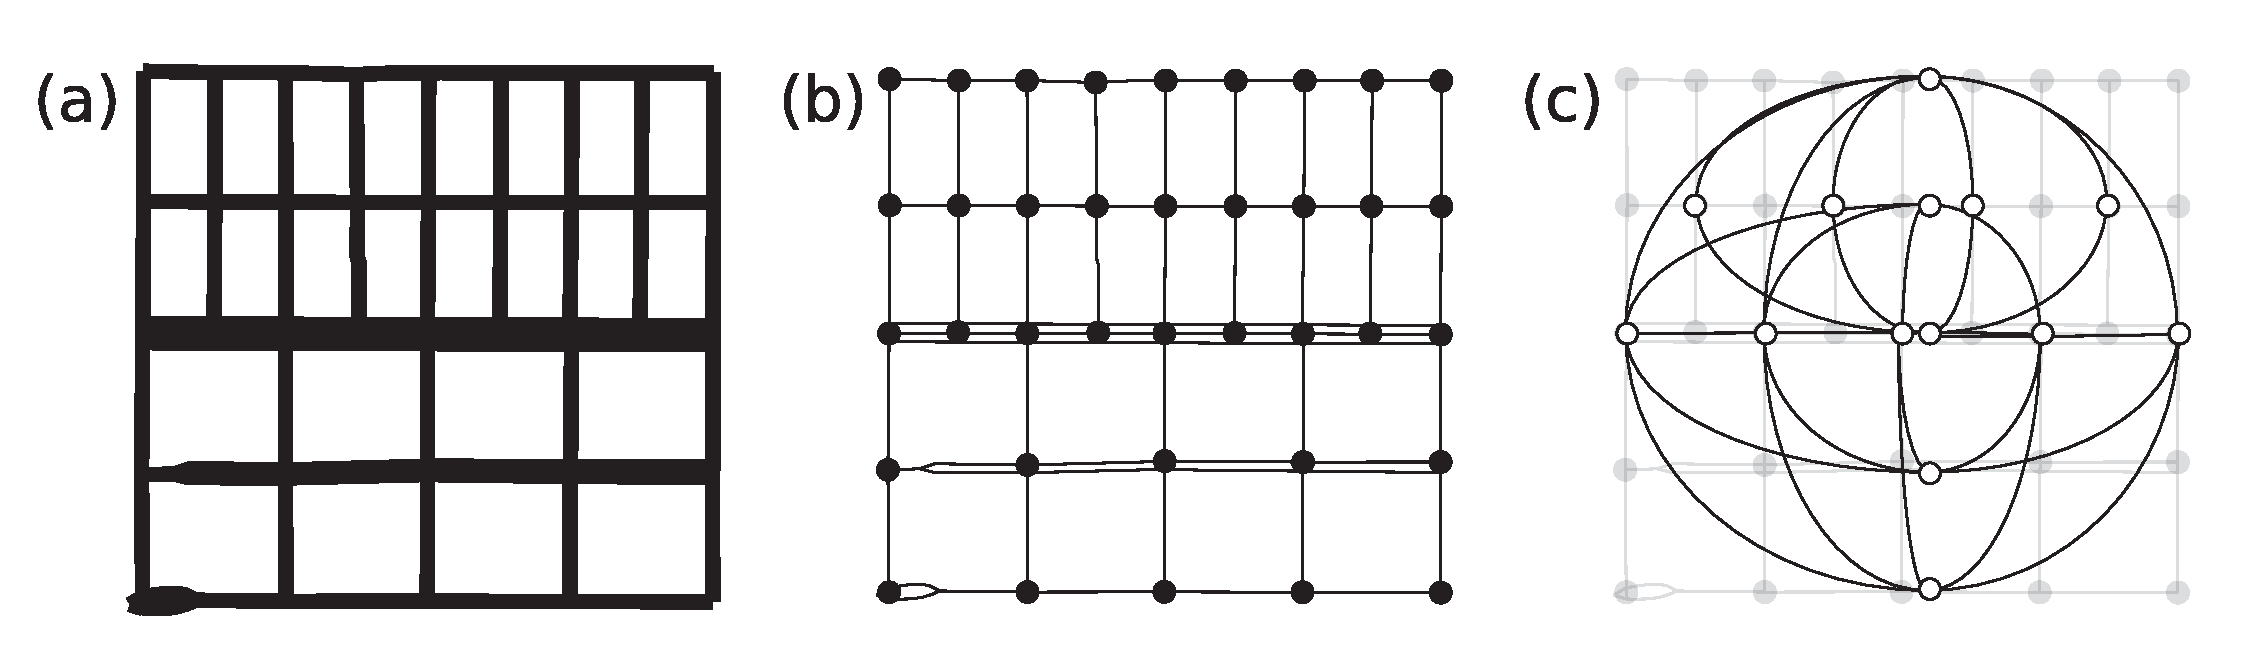
\includegraphics[width=\textwidth]{images/introduction/networks.pdf}
	\caption[Network representation of a city]{\textbf{(a)} Schematic street plan representation. \textbf{(b)} Primal representation of a street network, intersections are represented as nodes, and streets as edges. \textbf{(c)} Space syntax representation of a city. Continues streets mapped as nodes, and edges between intersecting streets.}
	\label{fig:networks}
\end{figure*}


%Street networks
Over the last decades, networks have emerged as a versatile tool to understand, map and visualize the interconnected architecture of a wide range of complex systems, from social systems to biology~\cite{albert2002statistical, dorogovtsev2002evolution, newman2003structure, boccaletti2006complex}, and in particular spatially embedded ones~\cite{barthelemy2011spatial}. When modelling a city as a network, there are two approaches. First, intersections can be mapped as nodes, and the streets (or any other mobility infrastructure) as edges~\cite{porta2006primal}. Following this approach it is possible to replicate the city's structure as a planar network~\cite{Boeing2020Planarity} (see Figure~\ref{fig:networks}~(a-b)). On the other hand, it is possible to model a city as a network following space syntax theory~\cite{hillier1976syntax} in which the streets are mapped as nodes depending on their continuity, and intersections are edges (see Figure~\ref{fig:networks}~(c)). Although the space syntax theory is useful to map relations between spaces/streets, it fails to capture the morphological properties of cities~\cite{batty2004new}. Along this thesis we will work with the primal representation of urban networks, considering intersections as nodes, and streets, sidewalks, or bike paths as edges connecting the nodes. As this network representation allow us to capture the urban structure and provide us with a framework to analyze it and compare multiple layers systematically.

Cities as networks have been extensively studied in the field of Network Science, first from a single-layer perspective, while more recently with a multilayer perspective, with special attention to transportation networks~\cite{lin2013complex,barthelemy2011spatial,ding2019application}, focusing on topological properties~\cite{jiang2004topological,cardillo2006structural,barthelemy2008patterns,batty2008size,barthelemy2011spatial,strano2013comparative,louf2014typology,boeing2020multiscale}, centrality metrics~\cite{crucitti2008centrality,Boeing2020Planarity,kirkley2018structural}, and growth processes~\cite{makse1995growth,strano2012evolution}. Other topics include the impact of the street networks on pedestrian volume~\cite{hajrasouliha2015connectivity}, accessibility and vitality of cities~\cite{denadai2016death,biazzo2019accesibility}, resilience of transportation networks~\cite{baggag2018resilience,ferretti2019resilience}. These recent approaches can be seen as the beginning of emerging fields such as the Science of Cities or Urban Data Science, which exploit new large-scale urban datasets with quantitative tools from physics, geoinformatics, and data/network science~\cite{batty2013new,resch2019hds}.

%Multimodal transportation and networks
When using networks to represent transportation systems~\cite{lin2013complex}, nodes can represent the stations of the system, and links the direct connections between such stations. However, in real world scenarios, the transportation systems are composed of multiple transportation options, such as subways, buses, tramways, and dedicated pedestrian and cyclist infrastructure. To be able to integrate these systems and represent the multimodal transportation options of a city, the system can be conveniently described by \textit{multiplex} or \textit{multilayer} networks~\cite{dedomenico2013mathematical,kivela2014multilayer,boccaletti2014structure,battiston2014structural}.

Having interconnected urban transportation infrastructure enables multimodal mobility. Multimodal mobility is the idea of the combination of modes in one trip. Naturally this happens in all cities - for example, a trip with a bus includes walking to and from a bus station. On the other hand, multimodal mobility can also be intentionally designed, such as bicycle-trains~\cite{geurs2016multi} or share mobility solutions to the last mile problem~\cite{shaheen2016mobility}. A multimodal transportation system offers the benefit of combining multiple transport modes and their advantages while avoiding their weaknesses, by connecting different modes through interfaces (e.g. stations) that facilitate transfers between the distinct services~\cite{vannes2002design}.

%Mobility and networks
The study of urban mobility combined with network science has not only been beneficial when dealing with infrastructures, as it has also been used to analyze human mobility dynamics~\cite{barbosa2018human}. The availability of data sets such as large-scale mobile phone data, have been used as proxies to understand mobility patterns in cities~\cite{gonzalez2008understanding}, finding predictable human mobility motifs related to socio-economic activities in cities. Understanding the interplay between infrastructure and dynamics is fundamental to tackle further multimodal planning challenges. Such as from the traveler's view, the need of processing large amounts of information when choosing convenient travel routes in multimodal systems~\cite{gallotti2016limits}. On the other hand, from the transport provider's perspective, when trying to achieve synchronization between different agencies and modes~\cite{barthelemy2016structure}.

In this thesis we build on current research to give original contribution to open questions such as the characterization of multimodal transport infrastructure, and how can large scale open data sets be used to identify similarities between cities based on their multimodal transportation options. Identifying universal patterns in urban development help plan systematic ways to build better cities. In that sense, it is important to address open research problems such as identifying strategies to improve sustainable mobility options in cities. Thus, we propose algorithmic tools to systematically connect different patches of urban bicycle infrastructure. Finally, we propose to leverage network science tools to create a framework that incorporates both: the urban physical structure, and practical knowledge from stakeholders, to measure liveability conditions.

\section{Aim and structure of the thesis}

The primary aim of this thesis is to build on previous research and contribute to the better understanding of the structural properties of multimodal transportation networks in urban areas. For that, we build on the tools and methods of network science to analyze the underlying complexity of urban mobility infrastructure.

In this thesis we begin focusing on the multimodal infrastructure network, first by providing a review of previous works related to multimodal transportation networks, and then giving an original contribution to the analysis of this specific type of system. In the following chapters, we focus on specific layers: first, by analyzing and giving an original contribution for the connectivity of bicycle infrastructure networks, and second, we propose and use a methodology to measure the urban quality of life as urban walkability taking the pedestrian infrastructure layer as the base for our calculations.

This thesis is structured in six chapters. In Chapter~\ref{ch:litReview}: We provide a review of previous works on multimodal transportation and mobility research from a complex systems' perspective. First we focus on the infrastructure and measures to quantify it, then on the mobility dynamics on top of these infrastructures, and finally we offer a review of available datasets and tools to analyze this specific type of networks.

In Chapter~\ref{ch:OverlapCensus} wWe make an original contribution to the field by proposing a method to extract the multimodal profile from a city's multiplex transport network. In this chapter, we apply our methods to fifteen cities, finding clusters of cities with similar multimodal infrastructure.

In Chapter~\ref{ch:BikeGrowth} we focus our attention on the bicycle layer of the multimodal network and propose algorithmic approaches to improve its connectivity. We find that focalized investment has the potential to rapidly improve the connectedness and directness of the bicycle infrastructure.

In Chapter~\ref{ch:LQI} we present a methodology to measure the quality of life in a city based on the pedestrian accessibility to amenities and services. We apply the methodology to Budapest and show how it can be used to capture inequalities in neighborhoods.

Finally, in chapter~\ref{ch:Conclusion}: We review the main contributions from this thesis, and outline future streams of work and open questions. 